% First set up the document structure and include the packages you would like to use
\documentclass[11pt]{article}
\usepackage{amsmath,times}
\usepackage{amssymb}
\usepackage[pdftex]{graphicx}
%\usepackage{subfigure,amsfonts}
\usepackage{array,tabularx}
\usepackage{hyperref}
\usepackage{epstopdf}
\usepackage{float}
\usepackage{listings}
\usepackage{color}
\usepackage[english]{cleveref}
\usepackage{graphicx}
%\usepackage{caption,subcaption}
\usepackage{caption}
\usepackage{subcaption}
\usepackage[ngerman]{babel} 
\usepackage[latin1]{inputenc}
\usepackage[T1]{fontenc}
\newcolumntype{C}[1]{>{\centering\let\newline\\\arraybackslash\hspace{0pt}}m{#1}}  % I define a column type for my data table to adjust the cell-width
%% ermöglicht Unter-Bilder in einer figure-Umgebung
%\usepackage{subfig}
%% Grafik-Dateien werden in den folgenden Ordnern gesucht
%\graphicspath{img/}
%% Grafikdateien haben die folgenden Endungen (höchste Priorität zu erst)
%\DeclareGraphicsExtensions{.pdf,.png,.jpg}
\usepackage[separate-uncertainty]{siunitx}
\sisetup{
    range-units = single,       % \SIrange soll die Einheit nur einmal anzeigen
    list-units  = repeat,       % \SIlist soll die Einheit wiederholen
}
% Begin your document, in this case I include a title page


%METAINFORMATIONEN
\title{PRESENTATION: Smartphones - circuit elements to handle digital signals}
\author{Nik Dennler}
%\subtitle{ATTENTION: This is not a to be published document. It is purely meant to be a guideline for an oral presentation and can contain citations and contents from others work without proper referencing.}
\date{November 16, 2016}

\begin{document}


\maketitle
\tableofcontents
\clearpage

%\tableofcontents  % optional - remove the * after the sections to get the section numbers
\section{Historical and current electric circuits and devices}
An electronic circuit is composed of individual electronic components, such as resistors, transistors, capacitors, inductors and diodes, connected by conductive wires or traces through which electric current can flow. The combination of components and wires allows various simple and complex operations to be performed: signals can be amplified, computations can be performed, and data can be moved from one place to another.

%\noindent
We differ between analogue circuits and digital circuits. The difference comes in the format of the signal that represents the carried information. 


\subsection{Analog circuits}
An analogue signal uses some attribute of the medium to convey the signal's information. For example, a compass uses the angular position of a needle as the signal to convey the information of the location of the magnetic north of the earth's magnetic field.  Electrical signals on the other hand may represent information by changing their voltage, current, frequency, or total charge. Analog electronic circuits are those in which the threshold of the current or voltage may vary continuously with time, corresponding to the information being represented. Analog circuitry is constructed from series and parallel circuits. The circuits are very commonly represented in schematic diagrams, in which wires are shown as lines, and each component has a unique symbol. 

%%Ref: \url{https://en.wikipedia.org/wiki/Electronic_circuit}}%
\begin{figure}[H]
\centering
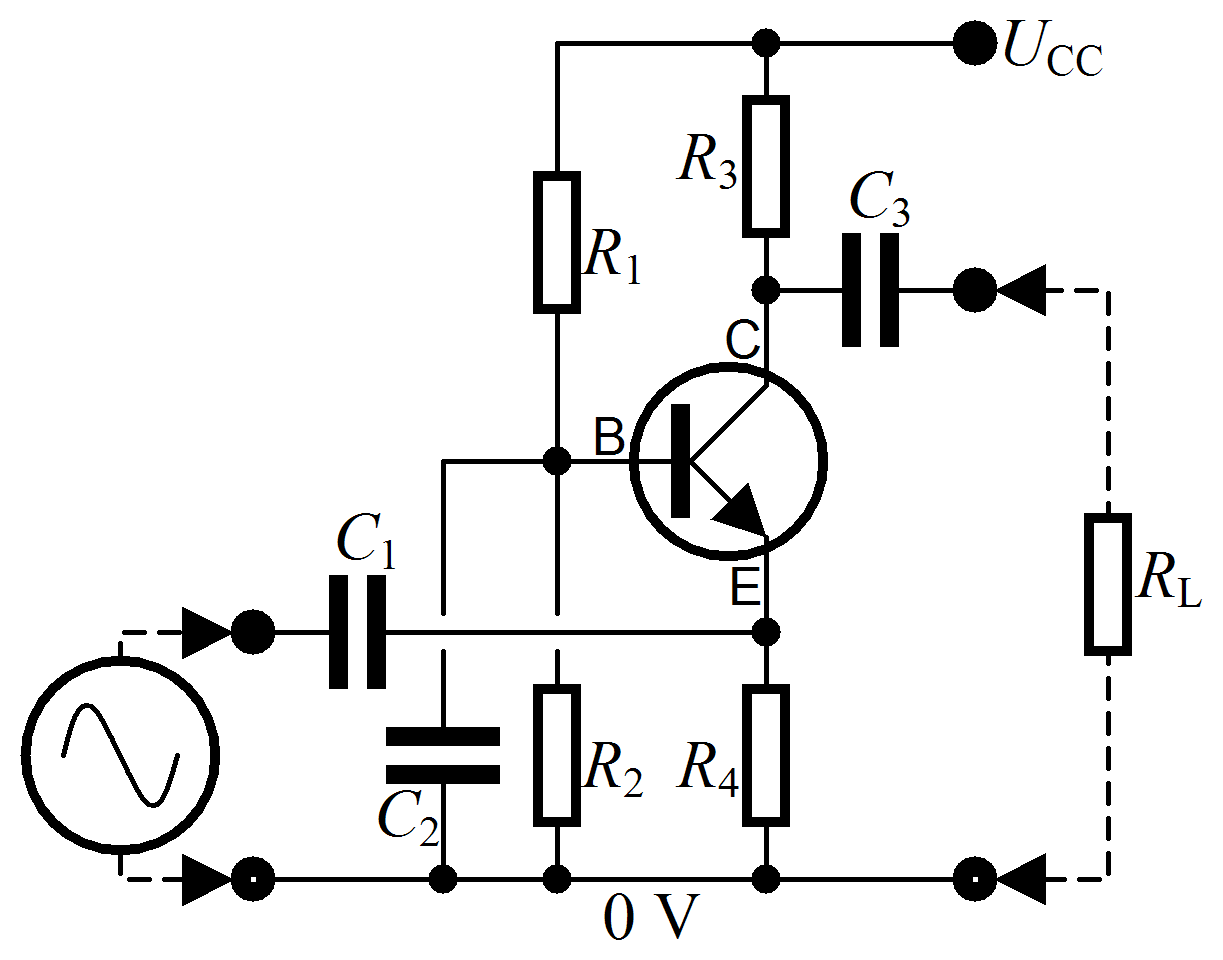
\includegraphics[width=0.6\textwidth]{ampcircuit.png}%
\caption{Circuit drawing of a simple amplifier}
\label{fig:amp}
\end{figure}

%\noindent
Analog circuit analysis employs Kirchhoff's circuit laws: all the currents at a node (a place where wires meet), and the voltage around a closed loop of wires is zero. 

(formula: Kirchhoff laws)

\subsection{Digital circuits}
In digital electronic circuits, electric signals take on discrete values to represent logical and numeric values, which then represent the information that is being processed. Every digital circuit is also a analog circuit, but it has just two potential levels in use. 
\subsubsection{Binary representation}
In most of the cases, binary encoding is used: one voltage represents a binary '1' and another voltage, usually a value near the ground potential, represents a binary '0'. Those binary digits, each of them called one 'bit', can then be used to represent numbers and characters and therefore to carry information. The binary code was invented and first used by Gottfried Leibniz in 1679, so Leibniz can somehow be considered as the first modern coder ever. 

%$table: http://binarynumbersa.blogspot.ch/2012/02/representation-of-binary-numbers.html$

%https://en.wikipedia.org/wiki/Binary_code#/media/File:Gottfried_Wilhelm_von_Leibniz.jpg$
\begin{figure}[H]
\centering
\begin{minipage}{0.5\textwidth}
%  \centering
  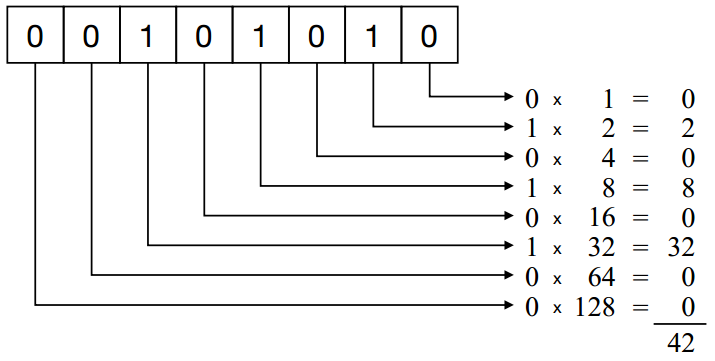
\includegraphics[width=1\textwidth]{binary.png}%
  \caption{Binary representation of one bit}%
  \label{fig:binary}
\end{minipage}%
\begin{minipage}{.4\textwidth}
  \centering
  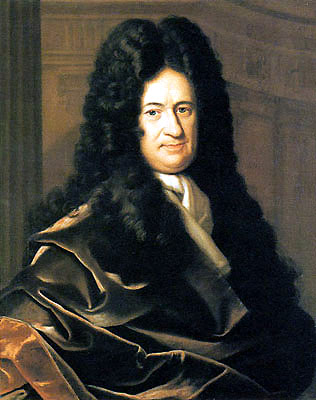
\includegraphics[width=0.8\textwidth]{leibniz}%
  \caption{Painting of Gottfried Leibniz}%
  \label{fig:leibniz}
\end{minipage}
\end{figure}

\subsubsection{Bool Algebra and logical circuits}
To understand how a processor can actually perform calculations and follow algorithms, some knowledge about Boolean logic has to be obtained first. We translate the digit '1' to True and the digit '0' to False. Now, how are binary signals worked with? In the first half of the 19. century did George Boole had an answer to that question as came up with the Boolean algebra, which defines three main operations: 

%\noindent
The conjunction: $a\land b$ is $True$ if and only if $a$ is $True$ and $b$ is $True$.\\
The disjunction: $a\lor b$  is $True$ if and only if $a$ is $True$ or $b$ is $True$ or $a\wedge b$ is $True$.\\
The negation:  $\neg a$ is $True$ if and only if $a$ is $False$. 

%\noindent
Those operations can be represented in so called truth tables as follows. We choose here again the $1 / 0$ representation.

\begin{table}[H]
\centering
\begin{tabular}{c|c|c|c|c}
\textbf{$a$} & \textbf{$b$} & \textbf{$a\land b$} & \textbf{$a\lor b$} & \textbf{$\neg a$} \\ \hline
0          & 0          & 0            & 0            & 1           \\
1          & 0          & 0            & 1            & 0           \\
0          & 1          & 0            & 1            & 1           \\
1          & 1          & 1            & 1            & 0          
\end{tabular}
\caption{truth table}
\label{tab:truth}
\end{table}

%\noindent
The operations of the Boolean Algebra are Associative, Commutative and Distributive. They have a Neutral, an Inverse and a Zero element. One can easily imagine, that those operations can be combined and added in number to create more complex calculation operators. This is actually exactly what happens in our computers, servers and smartphones, of course on a very large scale. 
So, how can those abstract boolean operators be realised to be implemented a digital circuit?
\subsubsection{Vacuum tubes}
A vacuum tube is a device that controls electric current between electrodes in an evacuated container. Vacuum tubes rely mostly on thermionic emission of electrons from a heated cathode. (There are also types of vacuum tubes that rely on the photoelectric effect, called Phototubes.) By thermionic emmission, also known as the Richardson-Edinson-effect, we mean that electrons of a metal gain enough energy through heating to leave its oxide surface. 
%2D sketch of diode with positive and negative voltage
%https://en.wikipedia.org/wiki/Thermionic_emission#/media/File:EdisonEffect.svg
\begin{figure}[H]
\centering
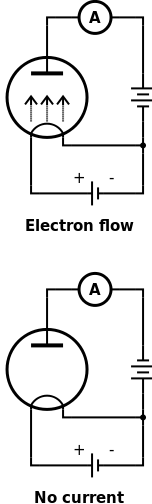
\includegraphics[width=0.3\textwidth]{edisoneffect.png}%
\caption{Eddison effect}%
\label{fig:edison}
\end{figure}


Richardson described the effect quantitatively and came to the following equation for the resulting current density $J$ of the leaving electrons:

\begin{equation} 
\label{eq:J}
J=A\cdot T^2 \cdot e^{-\frac{W_e}{k \cdot T}}
\end{equation}

\noindent
Here is $T$ the absolute temperature, $W_e$ the work function of the electrons, $k$ the Boltzmann constant and $A$ the Richardson constant.

%\noindent
The first functional vacuum tube with two elements was invented by John Fleming in 1904, it will later be known as the diode. A diode is a two-terminal component that conducts electricity primarily in one direction. The Fleming diode workes as follows: The cathode is heated, either directly through a flowing current or indirectly, and starts to emit electrons. Through the potential difference between the cathode and the anode are the electrons accelerated towards the anode. They are absorbed and the resulting current can be measured.


%\noindent
Three years later, in 1907, the inventor Lee de Forest patented a bulb with the same contents as the Fleming diode, except for an added electrode. The electrode acts as a grid between the cathode and the anode; depending on the grid-voltage there are more or less electrons flowing from the cathode to the anode. In this way it can be used to amplify a signal layed on the grid-electrode by modulating the anode-cathode-current. This device, known as the \textit{Audion}, was the first successful electronic amplifier.
%3Ddiode
%https://en.wikipedia.org/wiki/Vacuum_tube#/media/File:Diode-english-text.svg
%3Dtriode
%https://en.wikipedia.org/wiki/Vacuum_tube#/media/File:Triode-english-text.svg
\begin{figure}[H]
\centering
\begin{minipage}{0.3\textwidth}
  \centering
  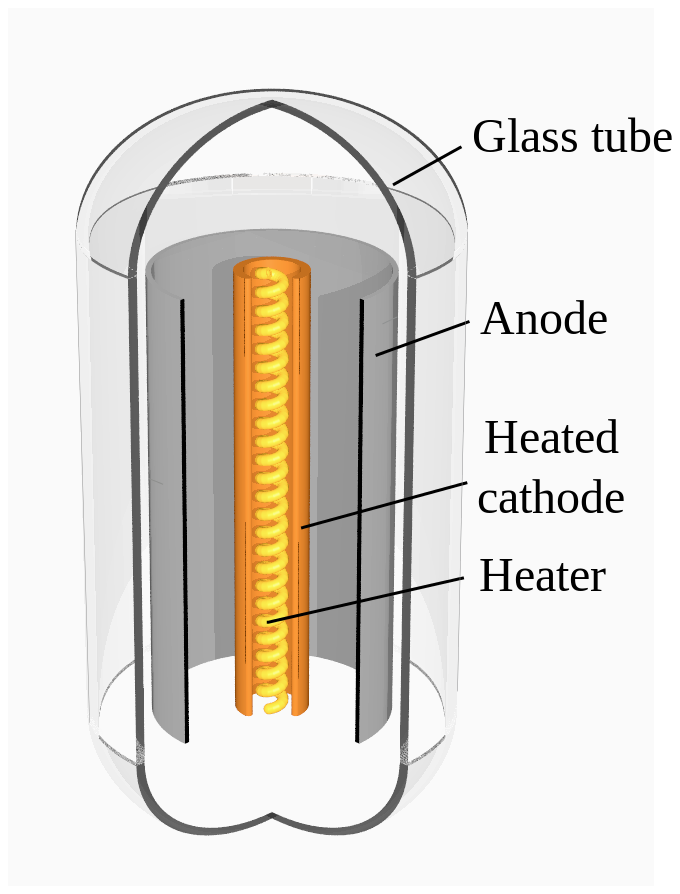
\includegraphics[width=0.8\linewidth]{diode.png}%
  \caption{3D Diode}%
  \label{fig:diode}
\end{minipage}%
\begin{minipage}{.3\textwidth}
  \centering
  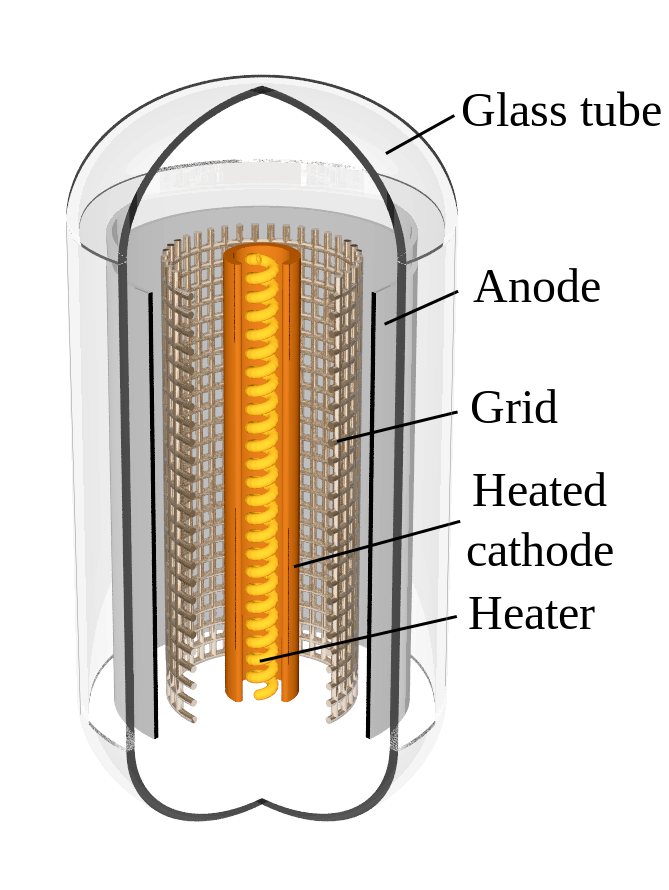
\includegraphics[width=0.8\linewidth]{triode.png}%
  \caption{3D Triode}
  \label{fig:triode}
\end{minipage}
\end{figure}

%\noindent
The triode made it possible to realize the first transcontinental telephone connection (1915) and gave rise to the electronics industry. In 1947, The computer \textit{ENIAC} was built in the United States to calculate artillery projectile trajectories and it was all based around 18'000 vacuum tube diodes and triodes. The computer was able to perform 5000 additions or subtractions per second, 385 multiplications per second, 40 divisions per second or 3 square root calculations per second. It weighted around 27t, was 30 meters long and consumed around 150kW of power. In relation, current notebooks consume between 20 and 50W. 
%%picture ENIAC
%https://en.wikipedia.org/wiki/ENIAC
\begin{figure}[H]
\centering
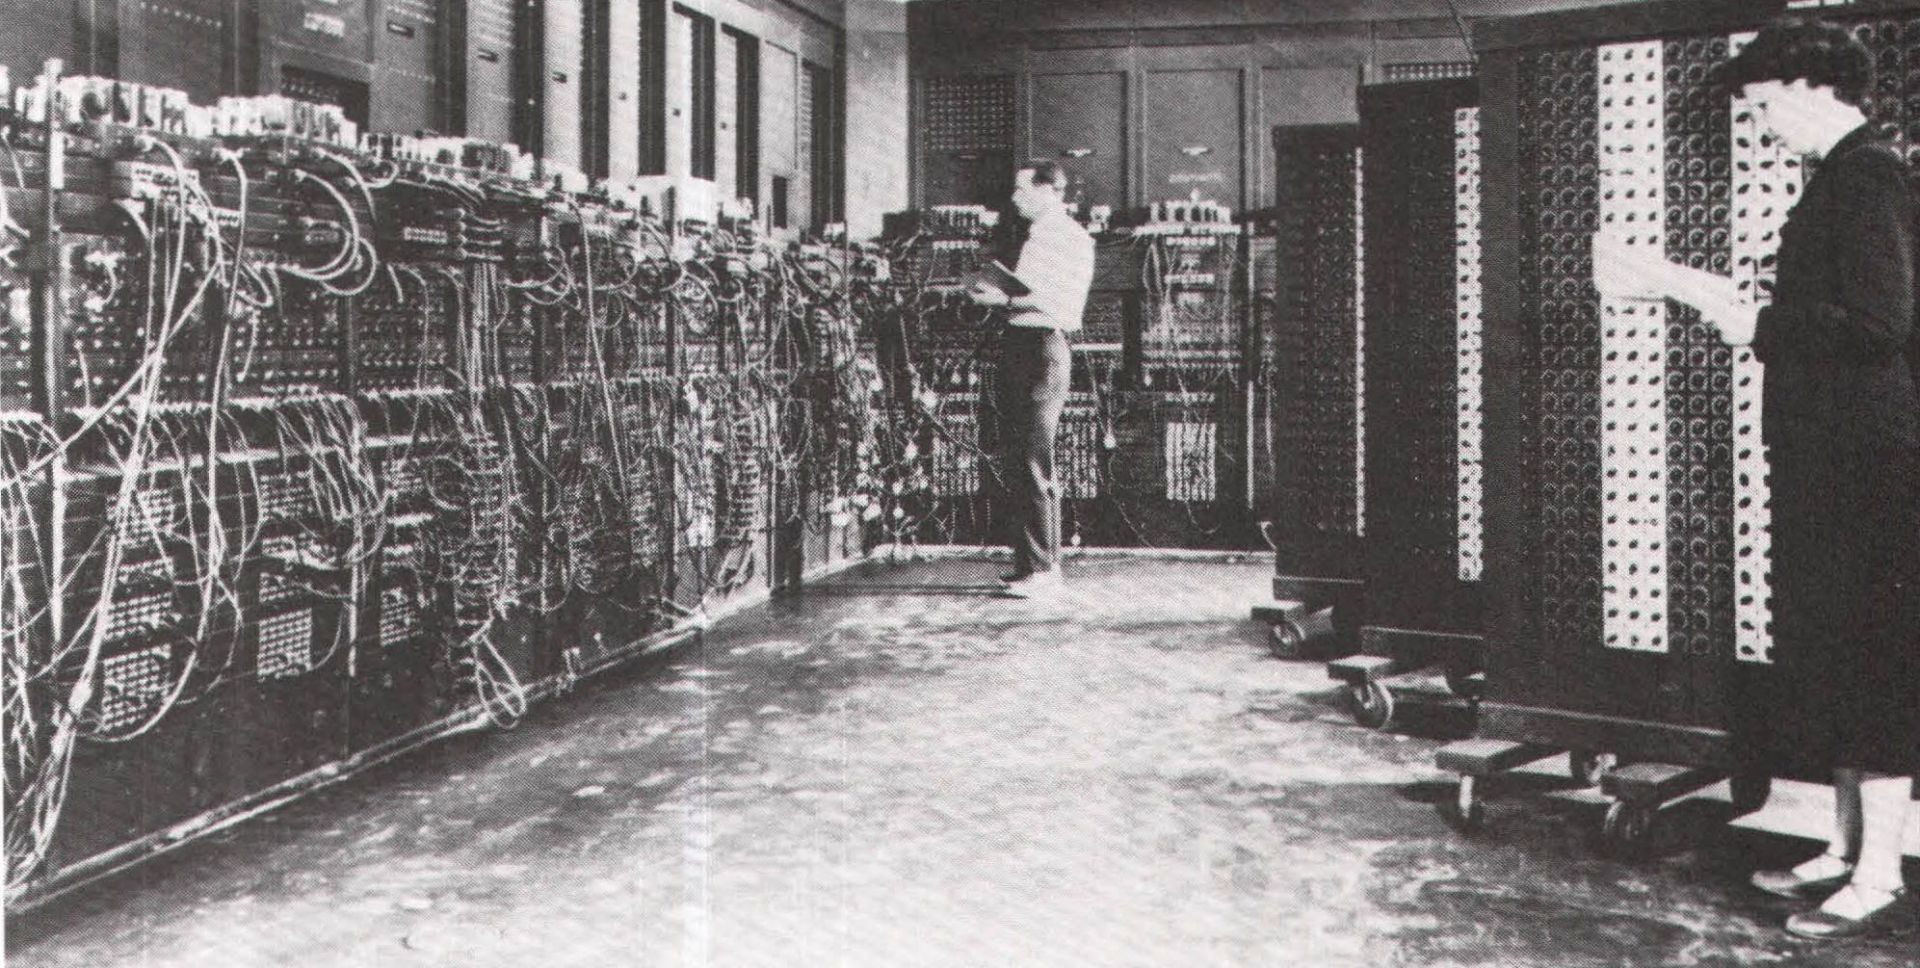
\includegraphics[width=1\textwidth]{eniac}%
\caption{ENIAC computer}
\label{fig:eniac}
\end{figure}

Nowadays the vacuum tube is not so common anymore, but it is still used in Photomultipliers and in high end audio devices.

\subsubsection{Transistors}
The vacuum tube got mainly replaced by the transistor - a triode based on semiconductors. In 1934 did the German physicist Oskar Heil invent the first silicon based field effect transistor. Transistor is short for transfer resistor; a electric resistance that can be controlled by electric current. It can either be used as a signal amplifier or as an On/Off-switch, which gives us the desired characteristic for our digital circuit component. The device became quickly to the most important active component of electrical circuits and can, at least in my opinion, be considered as the number one invention of the 20. century. In an electrical circuit looks the symbol for a transistor like this:

%http://www.engineersblogsite.com/wp-content/uploads/2013/02/Transistor-diagram.jpg
\begin{figure}[H]
\centering
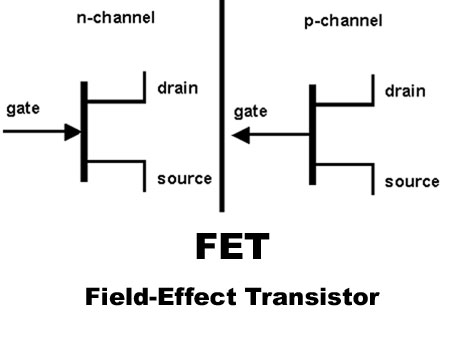
\includegraphics[width=0.7\textwidth]{transistor}%
\caption{transistor}
\label{fig:transistor}
\end{figure}



What the difference between the two transistors is and how the physics behind it works will be explained a bit later on.


\subsubsection{Logic gates}
meh? pictures of CompExp!

\subsubsection{Integrated circuits}
maybe later?

\newpage
\section{How does a Transistor work?}
Modern transistors are based on the semiconducting properties of silicon and germanium. 
\subsection{Semiconductors}
A semiconductor is a solid with an electric conductivity that lays between conductors and isolators. A pure semiconductor (also called intrinsic) at $OK$ has the properties of an isolator, but its conductivity rises with the temperature. This can be explained by observing the energy bands, which describe the combined Fermi-dirac-distribution of all electrons involved.

\begin{equation} 
\label{eq:Fermi}
f(E) = \frac{1}{1 + e^{\frac{E - \epsilon_F}{k \cdot T} } }
\end{equation}

At $OK$ all the electrons occupy a state in the valence-energy band (just below the Fermi energy $\epsilon_F$), which is then fully occupied, while the conducting band (just above $\epsilon_F$) is completely empty. By raising the temperature, the electrons get thermically excited and their probability of being in the conducting band rises. The electrons in the conducting band as well as the missing electrons in the valence band (called \textit{holes}) are contributing to the electric conductivity. 
%%image intrinsic conductor, electron bands, fermi dirac 
\begin{figure}[H]
\centering
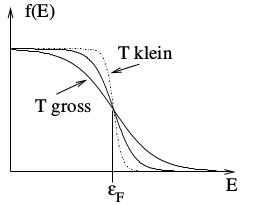
\includegraphics[width=0.5\textwidth]{fermi}%
\caption{Fermi-dirac distribution}
\label{fig:fermi}
\end{figure}


The special properties of semiconductors is given by the band gap between the valence and conducting band, which has to be big enough that there is no spontaneous conduction at low temperatures but small enough, that it conducts at the working temperature. If we compare the intrinsic conductivity of different materials, we get values as shown in this table: 

%%table of differenc intrinsic conductivites (Strauman skript)

\subsubsection{Doping}
For many applications the intrinsic conductivitiy of the named semiconducting materials is not enough. The process of infusing impurities into the matierial is called \textit{doping} and increases the number of free charge carriers (electrons and holes), which can lead to a much higher conductivity. Let's consider the example of silicon, which has a valence of 4. If we infuse a valence-5 atom like phosphor or arsen into the lattice on a spot, which was meant for a 4-valence atom, there will be an additional electron state, which is very weakly bound and can therefore contribute to the electric conduction. It's energy niveau is close to the conducting band, the fermi energy rises. We call the infused atom a \textit{donator} and the process \textit{n-doping}. 
%%Bild 8.19, Kittel
\begin{figure}[H]
\centering
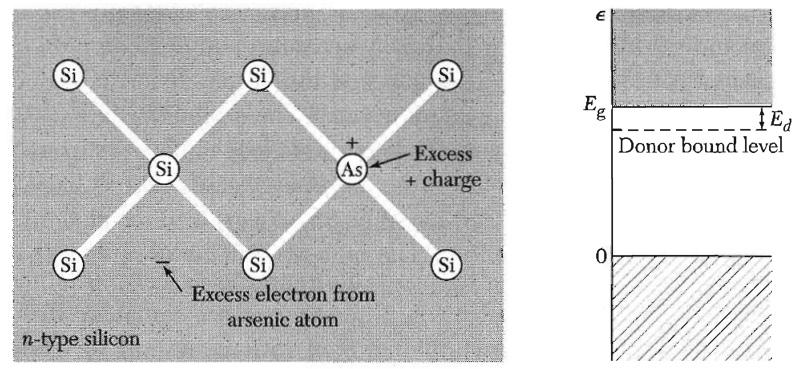
\includegraphics[width=0.9\textwidth]{donator}%
\caption{Donator: arsen-doped silicon}
\label{fig:donator}
\end{figure}

\noindent
If we do the opposite and infuse a valence-3 atom like bor, aluminum or gallium into the lattice, there will be an additional hole state, which lays close to the valence band and can easily bind an electron of the band. The Fermi energy sinks. Here we call the infused atom an \textit{acceptor} and the process \textit{p-doping}.   
%%Bild 8.20, Kittel
\begin{figure}[H]
\centering
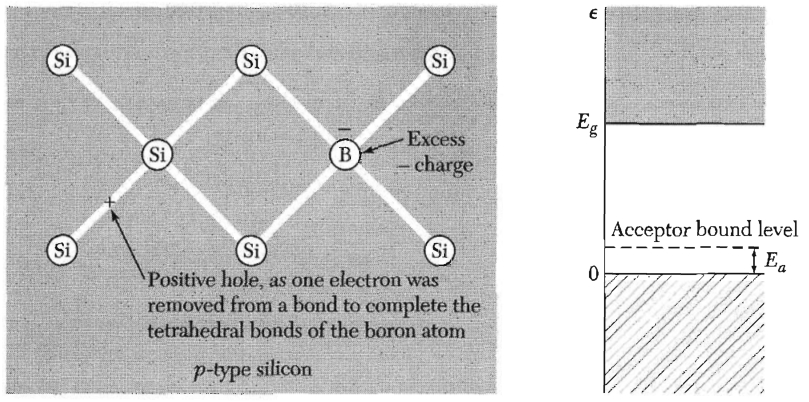
\includegraphics[width=0.9\textwidth]{acceptor}%
\caption{Donator: borium-doped silicon}
\label{fig:acceptor}
\end{figure}

\subsubsection{p-n junction}
So what happens when we bring together a p-doped and a n-doped material? The donator material conducts well because of its excess electrons while the acceptor materials conducts because of its excess hole states. But on the interface, on the \textit{p-n junction}, the excess holes from the p-area will diffuse to the n-area while the excess electrons from the n-area will diffuse to the p-area. Resulting there is a charge on the interface, which results in an electric field and therefore to a potential, that works against the diffusion. The result is an equilibrium in which the Fermi energy is constant. The sandwiched area is called \textit{depletion zone}; free electric charges cannot pass through it. 

%%https://en.wikipedia.org/wiki/P%E2%80%93n_junction#/media/File:Pn-junction-equilibrium-graphs.png
%%https://en.wikipedia.org/wiki/P%E2%80%93n_junction
\begin{figure}[H]
\centering
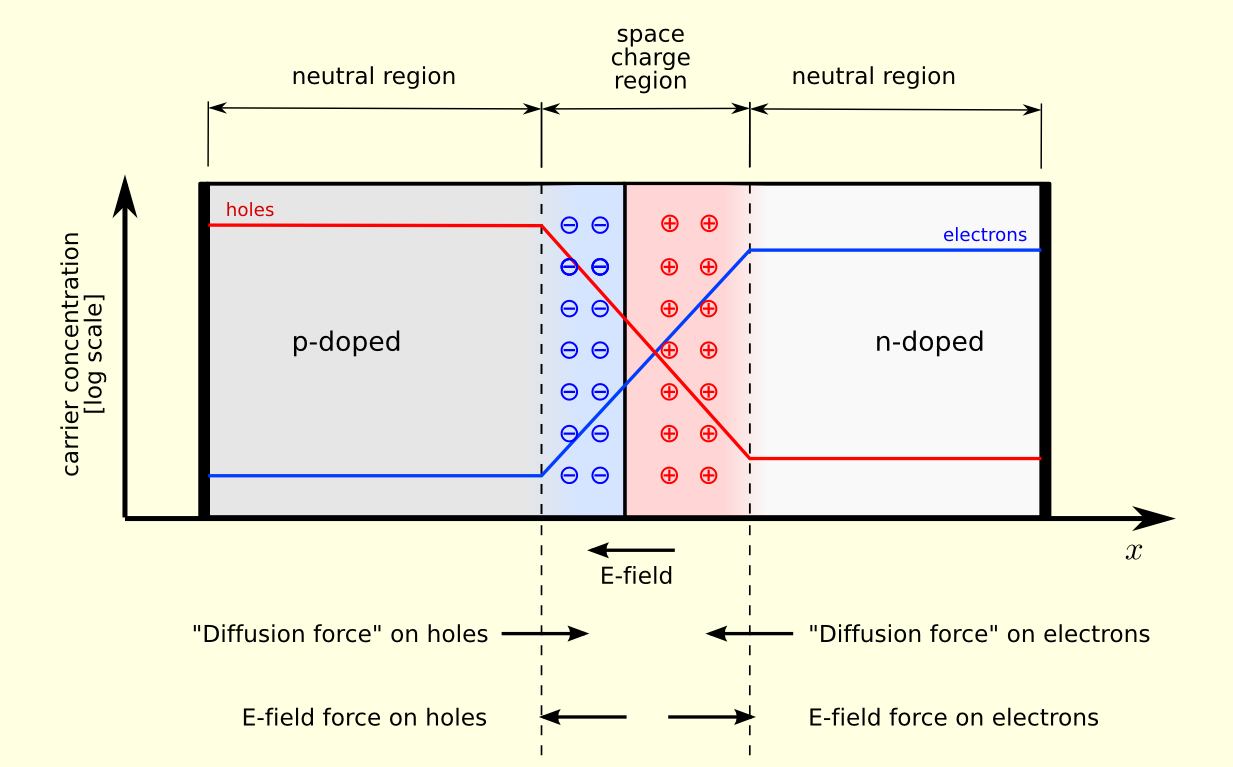
\includegraphics[width=1.0\textwidth]{pn_junction}%
\caption{diagram of a pn junction}
\label{fig:pn_junction}
\end{figure}

%\noindent
Now we want to apply a current to the junction. If the positive terminal is connected to the p-side and the negative terminal to the n-side of the junction, the holes in the p-type region and the electrons in the n-type region are pushed toward the junction and start to neutralize the depletion zone, reducing its width. As the width reduces shrinks the electric field, until the potential wall is small enough for the charges to pass through, resulting in a \textit{forward-bias} current. 

On the other hand, if we apply an opposite current, with the negative terminal connected to the p-side and the positive one to the n-side, the depletion zone grows. The \textit{holes} in the p-type material are pulled away from the junction, leaving behind charged ions and causing the width of the depletion region to increase. Likewise, because the n-type region is connected to the positive terminal, the electrons in the p-type region will also be pulled away from the junction, with similar effect. The increased potential barrier causes a high resistance to the flow of charge carriers, which results in the junction behaving as an insulator. 

What we have is therefore a diode based on semiconductor properties. The circuit symbol is 
%%https://en.wikipedia.org/wiki/Diode
\begin{figure}[H]
\centering
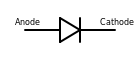
\includegraphics[width=0.3\textwidth]{diode_small}%
\caption{Circuit symbol of a diode}
\label{fig:diode_small}
\end{figure}
%%symbol diode

\subsection{Transistors}
As mentioned before, a transistor is a semiconductor device that has the same function as a triode: it has three terminals for connection to an external circuit and is used for amplifying or switching electronic signals and electrical power. A voltage or current applied to one pair of the transistor's terminals controls the current flowing through the other two terminals. In general, we differ between two types of transistors. 



\subsubsection{Bipolar Junction transistors (BJT)}
The first is the Bipolar Junction transistor. It is a combination of two junction diodes as seen before, and is formed of either a thin layer of p-type semiconductor sandwiched between two n-type semiconductors (a so called \textit{n-p-n transistor}), or a thin layer of n-type semiconductor sandwiched between two p-type semiconductors (a  \textit{p-n-p transistor}). The three terminals are defined by the three layer of semiconductor - an emitter, a base and a collector. It is controlled by a current on the base. It is called bipolar, because it used the conductivity of both electron and hole states.
%image p-n-p or n-p-n transistor
%%all transistor images by http://www.electronics-tutorials.ws
\begin{figure}[H]
\centering
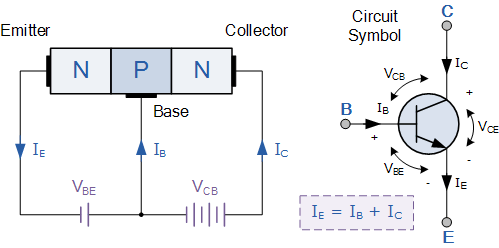
\includegraphics[width=0.8\textwidth]{npn}%
\caption{n-p-n transistor}
\label{fig:npn}
\end{figure}

Let's consider the n-p-n transistor. Usually we operate the emitter-base diode in \textit{forward-bias} and the collector-base diode in \textit{reverse-bias}. Electrons drift from the strongly doped emitter to the weakly doped, very thin base layer. The BC-depletion zone is reaching close to the CE-transision zone, so lots of electrons can drift into the BC-depletion zone, get pulled toward the collector and result a CE-current. We can now control the strengh of the CE- current by applying a current on the base, which will adjust the width of the p-zone. 
%diagram strauman skript, kennlinien n-p-n. 
\begin{figure}[H]
\centering
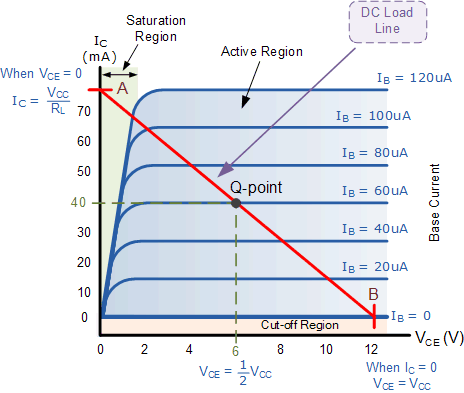
\includegraphics[width=0.6\textwidth]{kenn_npn.png}%
\caption{characteristic curve for a n-p-n BJT}
\label{fig:kenn_npn}
\end{figure}

The characteristic curve for a n-p-n BJT is shown in the graph above. We see that in the active region, the current flowing through the collector is not depending on the CE-voltage anymore. The base current alone controls how much current is flowing through the base. In the saturation region (green area) on the other hand is the CE-voltage so small, that the resulting current is actually coming from the open base-collector gate. The control is not working. 


*If the Bipolar NPN transistor is used as a On/Off switch, then the Cut-off region is used as the logical \textit{Off} and the saturation region, where there is almost no resistance, as the logical \textit{On}. But BJT's can not only be used as an On/Off switch, but also to amplify a small AC signal applied to the base terminal. Then it is important to know,  which CE-voltages and base-currents are necessary for a desired output collector current. The red line is called \textit{DC Load Line} and shows all the possible operating points for different values of applied base currents if we want to have a working signal amplifier. The Q-point gives us then the optimal point, where the output voltage can vary up and down. 


\subsubsection{Field effect transistors (FET)}
The second main type is the Field effect transistor, whose conductivity bases on only one type of state; either electron or hole. It is built up a bit differently than the Bipolar Junction transistor; it uses a gate, a source and a channel. Is is controlled by a voltage applied to the gate instead of a current.
%image FET, strauman skript\begin{figure}
\begin{figure}[H]
\centering
\begin{minipage}{.6\textwidth}
  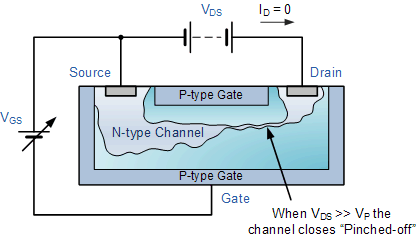
\includegraphics[width=1\linewidth]{jfet_closed}
  \captionof{figure}{JFET closed}
  \label{fig:jfet_closed}
\end{minipage}%
\begin{minipage}{0.6\textwidth}
  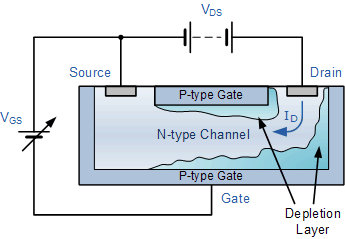
\includegraphics[width=.8\linewidth]{jfet_open}
  \captionof{figure}{JFET open}
  \label{fig:jfet_open}
\end{minipage}%
\end{figure}


The left image shows a blocked n-channel FET, which is built on a p-doped bulk. The voltage applied on the gate controls the current flowing from the source to the drain. For this example, if the source-drain-voltage is much bigger than the gate-voltage, electrons will collect just below the gate. The electrons will first compensate the holes of the p-bulk and built a depletion zone. The channel is closed and no current is flowing. But if the gate-voltage is increased, there will be a point when there are more electrons than hole states; the layer below the gate will become conductive and connect the source and the drain. 

\begin{figure}[H]
\centering
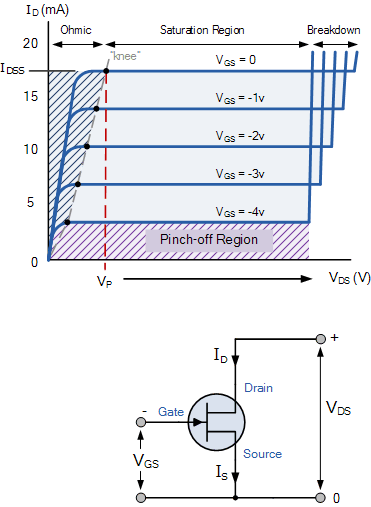
\includegraphics[width=0.6\textwidth]{kenn_jfet.png}%
\caption{characteristic curve for JFET}
\label{fig:kenn_jfet}
\end{figure}

In the cut-off region, where minimal voltage(or in this case even negative voltage) is applied to the gate, there is no current flowing at all. This region is in the switch-implementation used as the logical \textit{Off}. 
In the Ohmic region is the depletion layer of the channel very small and the transistor acts like a voltage controlled resistor. 
A larger current between source and drain results in a great potential drop and therefore in a space-dependent electric field, which becomes smaller close to the drain. The channel becomes thinner and limits the current flow, hence the name saturation zone. The transistor behaves as a constant-current source and can be used as a voltage amplifier. This region is also used as a logical \textit{On}. 
The breakdown region describes the point where the DS-voltage is high enough to cause the channel to break down and pass the maximum current. 

Actually there are many different types of Field effect transistors. The one we just looked at is called \textit{Junction FET (JFET)}, while the nowadays typically used is called \textit{Metal Oxide on Semiconductor FET (MOSFET)}. 

\begin{figure}[H]
\centering
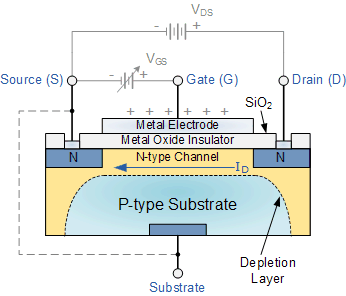
\includegraphics[width=0.6\textwidth]{mosfet.png}%
\caption{MOSFET}
\label{fig:mosfet}
\end{figure}


The MOSFET works very similar to the JFET, but it has a small layer of Silicium Oxide ($SiO_2$) as an insulator between gate and channel. The insulator plate can be thought of as one plate of a capacitor; it makes the input resistance of the MOSFET extremely high and prevents therefore any of the current flowing from the channel into the gate.   

\subsubsection{Differences, advantages and disadvantages of BJTs and MOSFETs}
Differences:
\begin{itemize}
 \item BJT has an emitter, collector and base, while a MOSFET has a gate, source and drain.
 \item BJTs uses both electron and hole states for conduction, while the channel in a FET depends on only one of them.
 \item The operation of MOSFET depends on the voltage at the oxide-insulated gate electrode, while the operation of BJT is dependent on the current at the base.
 \item The BJT is less complex than the MOSFET and was therefore preferred in earlier years.
 \item The BJT is less sensitive for damages in the installation. The MOSFET, due to its high capacity insulator layer, is very vulnerable to electrostatic damage.
 \item Due to the insulator layer does the MOSFET have much less current leak through the base than the BJT, which leads to less noise. 
 \item Because the MOSFET is voltage controlled, there is no additional power draw after the gate is opened or closed. Therefore it is more power efficient and can be used better on small scale. 
 \item The MOSFET is more resistent against radiation than the BJT. 
 \item BJTs are preferred for low current applications, while MOSFETs are for high power functions.
 \item Nowadays, if in digital and analog circuits, MOSFETs are considered to be more commonly used than BJTs.
\end{itemize}

\section{Future Solutions and Applications}
We have to ask ourself, what qualities do we want if we want to realize an optimal transistor?
\begin{itemize}
 \item Speed: A transistor should be as fast as possible, so we can make fast calculations. That means, that we want to have as much electron current flow from the source to the gate. One way to realize this is to make the path between source and drain as short as possible.
 \item Reliability: We want an exact transistor. Especially if we use it as a switch, we want to be sure that we can always distinguish well between OFF and ON. Therefore we want the ON/OFF current-ratio to be at least equal to 1000. 
 \item Low Power Consumption: We want a transistor that doesn't need much voltage. A big waste of power comes from the leak current, which can be redused by making the channel thinner and therefore the transistor smaller.  For a MOSFET we define the term of subthreshold-swing, which gives us the required gate-voltage to lower the potential wall 10 times (and therefore raise the current 10 times). The lower this number is, the less leak current we have. It is given by 
 \begin{equation}
 S_{s-th}=\frac{k_b\cdot T}{e}\cdot(1+\frac{C_D}{C_{ox}})
 \label{eq:subthresholdswing}
 \end{equation}
 where $T$ is the working temperature, $e$ the elementary charge, $C_D$ the depletion capacity and $C_{ox}$ the capacity of the insulating oxidation layer. If we let $C_{ox}$ go to infinity and plug in a temperature of $300K$, we get a minimum value of $60mV/dec$. So if we want our ON-current to be 1000-times larger, we need to have at least 240mV. 
 \item Size: Last but not least we want our transistor to be as small as possible, so we can fit as many of them on a processor. Also as visible in the above points, does it make sense to reduse the size to make the device faster and less power hungry.
\end{itemize}

\subsection{Moore's law}
After the invention of the transistor, a race about making smaller and smaller transistors started and different industrial branches participated in it. The advantage of small transistors is that more of the available resources (space) is used, that the speed is going up and the power consumption is going down. Therefore the general goal was to decrease the cost-optimal number of transistor per circuit element. The optimum is achieved by finding the balance of not wasting available space still not get into technical problems that arise with a too high transistor density. 
%%picture cost optimum
%https://de.wikipedia.org/wiki/Mooresches_Gesetz#/media/File:Mooresches_Gesetz.svg
%https://en.wikipedia.org/wiki/Moore%27s_law
\begin{figure}[H]
\centering
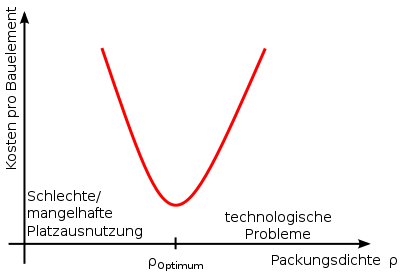
\includegraphics[width=0.5\textwidth]{moore_optimum}%
\caption{Cost optimum}
\label{fig:moore_optimum}
\end{figure}

\textit{Moore's Law} is a thumb-rule first proposed in 1965 by Gordon Moore that describes the time development of the optimal silicon transistor density. He predicted 50 years ago, that the number of transistors per area in a integrated circuit will double every two years. If we plot the most common transistor count per square centimeter for every year, we see, that we was quite right. 
%%picture moore's law
%https://en.wikipedia.org/wiki/Moore%27s_law
\begin{figure}[H]
\centering
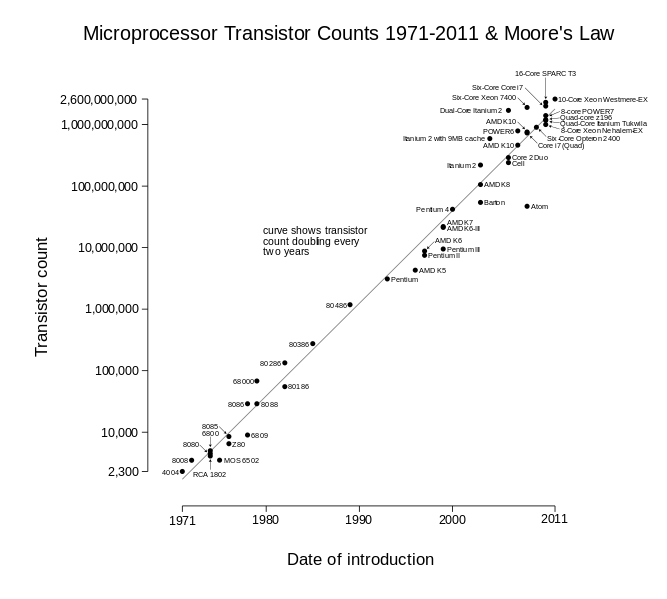
\includegraphics[width=0.9\textwidth]{moore}%
\caption{transistor count per IC for each year}
\label{fig:moore}
\end{figure}

The \textit{Intel 4004}-processor produced in 1971 was working with 2300 transistors, while the \textit{X-Box One} system chip produced in 2012 contained already 5'000'000'000 Transistors.

To be fair, Moore's proposal became eventually a self-fulfilling prophecy; the industries use his estimate to guide their research and production pace. For example in the year 2005, the most common chips produced had transistors of size between 130nm and 90nm, in preparation to mass production was already the 65-nm technique and in the lab was researched in structural sizes of around 40nm.
\subsection{Wo ist Schluss? Tunnel effect?}
The question automatically arises: Does it stop or will it go on forever? The answer is; it depends. If we only consider silicon based MOSFET transistors, then yes, the curve will flatten down and come to a count, where transistors just don't get smaller. The smallest mass-produced transistors right now are around 14nm (\textit{Intel 22-core Xeon Broadwell-E5}), where the size of one atom is between 0.1 and 0.5 nm; so we're getting closer to the atomic scale. This hosts various problems, where one of them is the tunnel current, occuring due to the quantum tunneling. A quick reminder: quantum tunneling refers to the quantum mechanical phenomenon where a partice tunnels through a barrier that it classically could not pass. 

%animation tunnel effect

Let's look at the metal-oxide-semiconductor field-effect transistor (MOSFET) to make this point clearer: If we want to decrease its size, we also have to decrease the oxide insulation layer. This will raise the probability of electrons tunneling through the isolator between the gate and the channel. This leads first to a substantial power drain, then to frequent loss of information and later to a complete useless logic gate. Silicone industry companies like \textit{Intel} assumes that 5 nanometers will be the last benchmark in size if only silicon transistors are taken in consideration. To make functional MOSFETs smaller than that won't be possible due to the excess in tunnel current. 

\subsection{UTBSOI and FINFET}
An Ansatz to make transistors better and smaller, is to thin the channel and therefore to bring the gate closer to the drain. When a transistor is off, the drain’s electric field can take one of two paths inside the channel to zero-voltage destinations. It can propagate all the way across the channel to the source, or it can terminate at the transistor’s gate. If the field gets to the source, it can lower the energy barrier that keeps charge carriers in the source from entering the channel. But if the gate is close enough to the drain, it can act as a lightning rod (Blitzableiter), diverting field lines away from the source. This cuts down on leakage, and it also means that field lines don’t penetrate very far into the channel, dissipating even more energy by tugging on any stray carriers.
\begin{figure}[H]
\centering
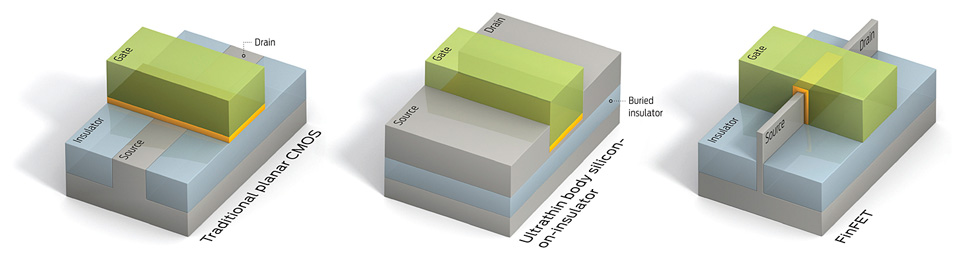
\includegraphics[width=1\textwidth]{fix_solutions}%
\caption{a) CMOSFET   b) UTB SOI   c) FinFET}
\label{fig:fix_solutions}
\end{figure}
\subsubsection{Ultrathin Body Silicon on Insulator (UTB SOI)}
The UTB SOI has an ultra-thin layer of insulator, called the buried oxide, positioned on top of the base silicon. Then, a very thin silicon film implements the transistor channel. Thanks to its thinness, there is no need to dope the channel, thus making the transistor Fully Depleted. On top of the channel comes again the oxide which insulates the controlling gate. The difference can be seen again in the following pictures:
%%www.st.com/.../FD-SOI/learn-more-about-fd-soi.html
\begin{figure}[H]
\centering
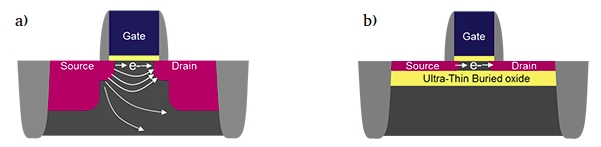
\includegraphics[width=1.1\textwidth]{UTBSOI}
\captionof{figure}{a) Bulk MOSFET   b) UTB SOI}
\label{fig:UTBSOI}
\end{figure}

%www.st.com/.../FD-SOI/learn-more-about-fd-soi.html
\begin{figure}[H]
\centering
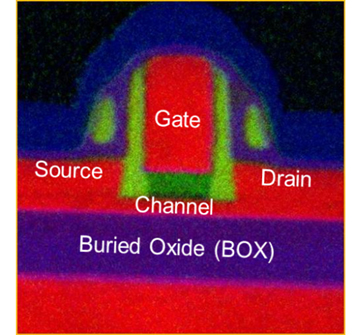
\includegraphics[width=.3\textwidth]{UTBSOIem}
\captionof{figure}{UTB SOI under the electron microscope}
\label{fig:UTBSOIem}
\end{figure}

\subsubsection{From 2D to 3D: FinFET}
The FinFET has a 3D architecture which also helps to bring the gate closer to the drain. They use a conducting channel that rises above the level of the insulator, creating a thin silicon structure, shaped like a fin, which is called a gate electrode. This fin-shaped electrode allows multiple gates to operate on a single transistor. FinFETs exhibit more drive current per unit area than their two-dimensional counterparts and are therefore faster or less power hungry. 

\subsection{Tunnel FET (TFET)}
But also those implications have their limits and actually still have to obey the subthreshold rule state before. So new technologies have to be found, for which some candidates are: Tunnel FETs, Photoemission-based microelectronic devices, Gallium arsenide transistors, Mott insulators, organic semiconductors, graphene and many more.

\begin{figure}[H]
\centering
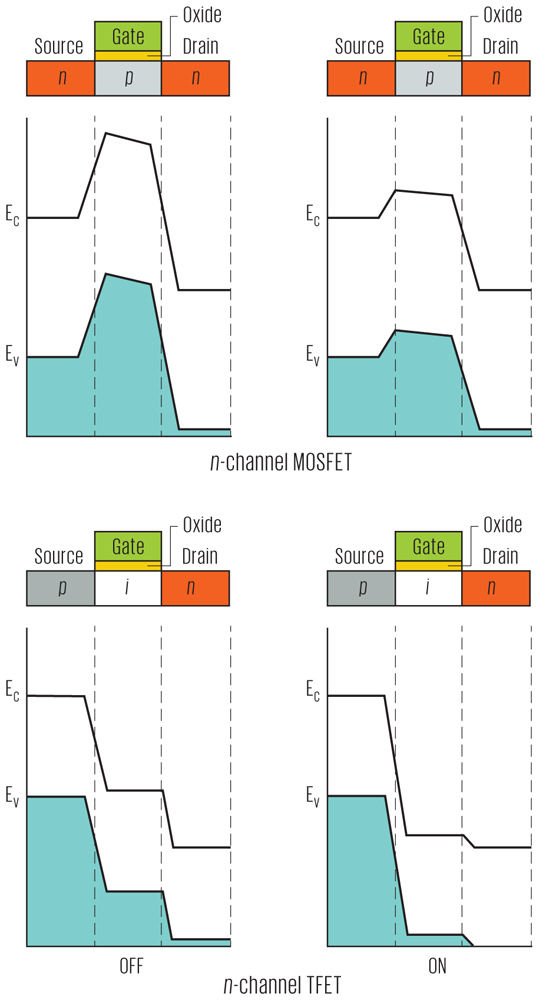
\includegraphics[width=0.6\textwidth]{MOSFETvsTFET}%
\caption{a) MOSFET   b) TFET}
\label{fig:MOSFETvsTFET}
\end{figure}

One new approach, which would actually use quantum tunneling for its benefit, is the Tunnel Field Effect Transistor (TFET). It's structure is very similar to the MOSFET, it is also built by adding together two junctions. But this time, a p-i junction and an i-n junction are used, where the 'i' stands for an intrinsic area, meaning that there are equally as many electrons and hole states. The fundamental switching mechanism is very different though. 


Again for a MOSFET: Electrons are in the conducting band while holes are in the valence band. In OFF-state, the electrons and the holes cannot pass the big potential wall provided by p-doped area. In ON-state this potential wall is being lowered by a voltage on the gate and the electrons resp. holes can pass. The conduction effect is due to thermionic emission.


For the TFET: All charge carriers (electron\&holes) are initially (OFF-state) in the valence band. By lowering the energy level of the intrinsic area with an applied gate-voltage, we make the tunneling potential wall narrower and allow the electrons to tunnel from the valence band to the conducting band and therefore setting the switch to an ON-state. Here the conduction is due to the quantum tunneling through the barrier. 

So what are the advantages and disadvantages of TFETs?
\begin{itemize}
 \item TFETs can have a much lower barrier with a thickness of around one atom. Therefore the transistor could be much smaller than MOSFETs. 
 \item TFETs are theoretically not limited by the MOSFET drain current subthreshold swing of about 60 mV/decade of current at room temperature. Actually in 2004, researches at IBM demonstrated first, that current swings below the MOSFET’s 60-mV-per-decade limit were possible. They produced a carbon nanotube TFET and got a value of 40 mV/decade. 
%%Image IBM 
 \item For quantum tunneling purposes it is much more effective to use materials with a direct band gap instead of indirect band gaps. Silicon has a indirect band gap, so to make TFETs effective, the industries would have to switch away from silicon first. This means, all the manufacturing processes would have to be changed, which comes with a big financial load. 
 \item By using those materials, the chances also rises that the electrons just tunnel straight from source to drain, which can become a problem if the channel length is shortened also. 
 \item 
%%image direct indirect band gaps 
\end{itemize}





\section{Sources}
\begin{itemize}
 \item Ch. Kittel, Einführung in die Festkörperphysik (Oldenbourg, Munich, 1999)
 \item U. Tietze \& Ch. Schenk, Halbleiter-Schaltungstechnik (Springer, Heidelberg, 2010)
 \item P.T. Landsberg, Solid State Theory (Wiley, New York, 1969)
 \item B. El-Kareh, Silicon Devices and Process Integration (Springer, New York, 2009)
 \item U. Straumann, Elektronik für Physiker (UZH, Zürich, 2005)
 \item \url{https://www.westfloridacomponents.com/blog/transistors}
 \item \url{http://www.electronics-tutorials.ws/transistor/tran_6.html}
 \item \url{http://www.vacuumtubes.net/How_Vacuum_Tubes_Work.htm}
 \item \url{http://spectrum.ieee.org/semiconductors}
 \item J. Appenzeller, Y.-M. Lin, J. Knoch, Band-to-Band Tunneling in Carbon Nanotube Field-Effect Transistors (IBM, New York, 2004)
 \item E. Forati, E. et al. Photoemission-based microelectronic devices. Nat. Commun. 7, 13399 doi: 10.1038/ncomms13399 (2016)
\end{itemize}


\section{questions to ask}

\subsection{Why silicon?}
periodic table, number 4, i.e. 4 empty 4 full 
\subsection{Avalanche breakdown in reverse bias}
\subsection{What happens if you operate the n-p-n transistor the other way around?}
\subsection{Advantages and disadvantages of BJT and FET?}
\subsection{Manufacturing processes}
\subsubsection{Photolithographic techniques}
\subsubsection{Logic gates}



\end{document}


\iffalse

\section{Set up}
\subsection{Mach-Zehnder interferometer}
The set up of the experiment is shown in \cref{fig:MZ}. The \emph{He-Ne} laser emits a photons beam of wavelength $\lambda$=632.8 nm. The beam passes through the rotating filters \emph{F1} and \emph{F2} (just one used in the present experiment), is reflected by the mirror \emph{S1} and is splitted by the beam-splitter \emph{BS1} in two beams of similar intensity. These beams are reflected by the mirrors \emph{S2} and \emph{B3} and meet again in the beam-splitter \emph{BS2}, from which a part of the photons reach the photomultiplier PMT, and the other part reachs the Charge-Coupled Device camera CCD (Pulnix TM-765) after being reflected by the mirror \emph{S4}. In front of the photomultiplier and of the CCD camera there are two boxes, which allow to set disc filters at the entrance of the sensors.
\begin{figure}[H]
\centering
\includegraphics[width=7cm]{img/MZ.png}%
\caption{Set-up of the experiment (from lab protocol)}%
\label{fig:MZ}
\end{figure}

\newpage
\subsection{Photomultiplier}
The photomultiplier is a photon detector which transforms the incoming photon in electric current. Its functioning is shown in \cref{fig:pmt}: the photons coming to the cathode release electrons by means of the photoelectric effect. Due to an applied voltage, these are attracted to the first dynode, where they release more electrons, which are attracted to the second dynode by the high voltage. The process is repeated from dynode to dynode, until a considerable electron current reaches the anode. The current flows through a resistance generating a voltae $V$, which can be measured. The current at the anode can be also visualized as function of the time with an oscilloscope.\\


\begin{figure}[H]
\centering
\includegraphics[width=10cm]{img/pmt.png}%
\caption{Sketch of the functioning of a photomultiplier, (from lab protocol)}%
\label{fig:pmt}
\end{figure}

\noindent
The relationship between the rate of detected photons $\frac{N_{\gamma}}{\Delta t}$ and the current generated in the photomultiplier is given by
\begin{equation} \label{pm}
\frac{N_{\gamma}}{\Delta t}=I\cdot G(V)\cdot Q_{\epsilon},
\end{equation}
where $I$ is the current, $G(V)$ is the gain of the multiplier that depends on the applied high voltage, and $Q_{\epsilon}$ is the quantum efficiency of the photomultiplier. The quantum efficiency $Q_{\epsilon}$ can be estimated from \cref{fig:grpmt} which was given by the manufacturer. For 350K and the wavelength $\lambda=532.8$ nm, it is approximately 0.5\%. 

\begin{figure}[H]
\centering
\includegraphics[width=9cm]{img/grpmt.png}%
\caption{Quantum efficiency of the photomultiplier as function of the wavelength for different materials}%
\label{fig:grpmt}
\end{figure}



\section{Theory}
\subsection{Important formulas}
The power of the emitted photon beam is given by
\begin{equation} \label{pow}
P=\frac{\Delta E}{\Delta t}=\frac{N_{\gamma}\cdot h\cdot c}{\Delta t\cdot \lambda},
\end{equation}
where $N_{\gamma}$ is the number of photons flowing in the interval $\Delta t$, $h$ is the Planck constant, $c$ the speed of light and $\lambda$ the wavelength of the photons. According to the laser manufacturer is $\lambda=\SI{632.8}{nm}$.
It follows that the number of emitted photons in the time interval $\Delta t$ is given by
\begin{equation} \label{N}
\frac{N_{\gamma}}{\Delta t}=\frac{P\cdot \lambda}{h\cdot c}.
\end{equation}
Since the path of the photons in the interferometer is of the order of magnitude of $L=\SI{30}{cm}$, the time needed by a single photon to pass through the interferometer is given by
\begin{equation} \label{time}
\Delta t=\frac{L}{c}\approx \SI{1}{ns}.
\end{equation}
According to the measurements, the power of the laser is $P_{0}=(5.16\pm0.01) mW$. The number $N_{0}$ of photon emitted in the time interval $\Delta t=\SI{1}{ns}$ can be calculated by using \cref{N}. We get $N_{0}= (1.643\pm 0.003)\cdot 10^{7}$ photons that are emmited by the source. The error was computed as
\begin{equation} \label{N_e}
\sigma_{N}=\SI{1}{ns}\cdot \frac{\lambda}{h\cdot c}\cdot \sigma_{P}.
\end{equation}
In order to observe the behaviour of a single photon in the interferometer, we have to reduce the power of the beam of a factor $T$, given by
\begin{equation} \label{T}
T_{t}=\frac{1}{N_{0}}\approx 6.08\cdot 10^{-8}.
\end{equation}
To this purpose, we let the beam pass through various filters of transmission coefficient $T_{i}$ before it reaches the sensors. The effective total transmission coefficient $T_{eff}$ is then given by
\begin{equation} \label{prod}
T_{eff}=\prod\limits_{i} T_{i}
\end{equation}
Thus, we can choose the filter combination leading to the desired total transmission coefficient $T_{t}$.\\
\subsection{Error propagation}
In general for errors do we use the Gaussian error propagation formula
\begin{equation}
(m_u)^2=(m_{x1} \cdot \frac{d_u}{d_{x1}})^2+(m_{x2} \cdot \frac{d_u}{d_{x2}})^2+...+(m_{xn} \cdot \frac{d_u}{d_{xn}})^2 .
\label{eq:error}
\end{equation}



\section{Procedure and measurements}
\subsection{Determination of the transmission coefficient of the components}
In order to reduce the flux of photons in the interferometer, we let the photons beam pass through various filters, whose transmission coefficient $T$ was determined experimentally. Moreover, since also the mirrors and the beam-splitters disperse a part of the incoming beam, we also measured the transmission coefficient of the various components of the experiment.\\
The power of the beam as ejected from the laser was measured as $P_{0}$=(5.16$\pm 0.01) mW$. At first we measured the transmission coefficient $T_{F}$ of the rotating filter \emph{F1}, which depends on the angle $\theta$ of its rotating component. The following table (\cref{tab1}) shows the power $P(\theta)$ measured between the rotating filter \emph{F1} and the mirror \emph{S1} as function of the angle $\theta$, and the corresponding transmission coefficient $T_{F}(\theta)$, computed as
\begin{equation} \label{t(theta)}
T_{F}(\theta)=\frac{P(\theta)}{P_{0}}.
\end{equation}
Accordingly, the corresponding error $\sigma_{T}$ was computed as
\begin{equation} \label{t(theta)_e}
\sigma_{T}=\sqrt{(\frac{1}{P_{0}}\cdot\sigma_{P_{0}})^{2}+(\frac{P(\theta)}{P_{0}^{2}}\cdot\sigma_{P(\theta)})^{2}},
\end{equation}
where $\sigma_{P_{0}}$ is the error on $P_{0}$ and $\sigma_{P}$ is the error on $P(\theta)$. The variations of the error on the power are due to the different accuracy of the power-meter for different power ranges.\\
The transmission coefficient as a function of the angle $\theta$ is shown in \cref{gr1}. 

\begin{figure}[H]
\centering
\includegraphics[width=11 cm]{img/gr1.png}
\caption{Transmission coefficient $T_{F}(\theta)$ of the rotating filter \emph{F1} as function of the angle $\theta$}
\label{gr1}
\end{figure}

\begin{table}[H]
\centering
\begin{tabular}{c| c| c}
angle $\theta$ [$\,^{\circ}$] $\pm 1\,^{\circ}$& power $P(\theta)$ [mW] & transmission coefficient  $T_{F}(\theta)$\\ \hline
0&	0.13$\pm 0.01$	&2.5(2)\\
10&	1.56(1)$\pm 0.01\cdot 10^{-3}$& 3.02$\pm 0.02\cdot 10^{-4}$\\
15&	0.69$\pm 0.01\cdot 10^{-3}$&	1.34$\pm 0.02\cdot 10^{-4}$\\
20&	0.79$\pm 0.01\cdot 10^{-3}$&	1.53$\pm 0.02\cdot 10^{-4}$\\
25&	0.92$\pm 0.01\cdot 10^{-3}$&	1.78$\pm 0.02\cdot 10^{-4}$\\
30&	1.10$\pm 0.01\cdot 10^{-3}$&	2.13$\pm 0.02\cdot 10^{-4}$\\
35&	1.31$\pm 0.01\cdot 10^{-3}$& 2.54$\pm 0.02\cdot 10^{-4}$\\
40&	1.43$\pm 0.01\cdot 10^{-3}$&	2.77$\pm 0.02\cdot 10^{-4}$\\
50&	1.94$\pm 0.01\cdot 10^{-3}$& 3.76$\pm 0.02\cdot 10^{-4}$\\
60&	2.57$\pm 0.01\cdot 10^{-3}$& 4.98$\pm 0.02\cdot 10^{-4}$\\
70& 3.86$\pm 0.01\cdot 10^{-3}$&	7.48$\pm 0.02\cdot 10^{-4}$\\
80& 6.35$\pm 0.01\cdot 10^{-3}$&	12.31$\pm 0.02\cdot 10^{-4}$\\
90& 10.82$\pm 0.01\cdot 10^{-3}$& 20.97$\pm 0.02\cdot 10^{-4}$\\
100& 18.32$\pm 0.01\cdot 10^{-3}$& 35.50$\pm 0.02\cdot 10^{-4}$\\
110& 24.8$\pm 0.1\cdot 10^{-3}$& 48$\pm 2\cdot 10^{-4}$\\
120& 39.1$\pm 0.1\cdot 10^{-3}$& 76$\pm 2\cdot 10^{-4}$\\
130& 54.2$\pm 0.1\cdot 10^{-3}$& 105$\pm 2\cdot 10^{-4}$\\
140& 76.0$\pm 0.1\cdot 10^{-3}$& 147$\pm 2\cdot 10^{-4}$\\
150&0.1114$\pm 0.0001$&	216$\pm 2\cdot 10^{-4}$\\
160&0.158$\pm 0.001$&	306$\pm 2\cdot 10^{-4}$\\
170&0.22$\pm 0.001$&    4.3$\pm 0.2\cdot 10^{-2}$\\
180&0.31$\pm 0.01$&	6.0$\pm 0.2\cdot 10^{-2}$\\
190&0.41$\pm 0.01$&	7.9$\pm 0.2\cdot 10^{-2}$\\
200&0.54$\pm 0.01$&	10.5$\pm 0.2\cdot 10^{-2}$\\
210&0.70$\pm 0.01$&	13.6$\pm 0.2\cdot 10^{-2}$\\
220&0,84$\pm 0.01$&	16.3$\pm 0.2\cdot 10^{-2}$\\
230&1.$\pm 0.01$&	19.4$\pm 0.2\cdot 10^{-2}$\\
240&1.25$\pm 0.01$&	24.2$\pm 0.2\cdot 10^{-2}$\\
250&1.69$\pm 0.01$&	32.7$\pm 0.2\cdot 10^{-2}$\\
260&2.55$\pm 0.01$&	49.4$\pm 0.3\cdot 10^{-2}$\\
270&4.52$\pm 0.01$&	87.6$\pm 0.4\cdot 10^{-2}$\\
280&4.96$\pm 0.01$&	96.1$\pm 0.4\cdot 10^{-2}$\\
290&4.84$\pm 0.01$&    93.8$\pm 0.4\cdot 10^{-2}$\\
300&4.68$\pm 0.01$&	90.7$\pm 0.4\cdot 10^{-2}$\\
310&4.54$\pm 0.01$&	88.0$\pm 0.4\cdot 10^{-2}$\\
320&4.51$\pm 0.01$&	87.4$\pm 0.4\cdot 10^{-2}$\\
330&4.45$\pm 0.01$&	86.2$\pm 0.4\cdot 10^{-2}$\\
340&4.41$\pm 0.01$&	85.5$\pm 0.4\cdot 10^{-2}$\\
350&4.40$\pm 0.01$&	85.3$\pm 0.4\cdot 10^{-2}$\\

\end{tabular}
\caption{Power $P(\theta)$ and transmission coefficient $T_{F}(\theta)$ of the filter $F1$ for different angles $\theta$}
\label{tab1}
\end{table}

\newpage
\noindent
As noted above, also the components of the interferometer disperse a part of the power; moreover we have to take in account that the photomultiplier and the CCD camera are reached respectively by approximatively one half of the resulting beam, In order to compute the transmission coefficient $T$ of the interferometer we have measured the power $P$ in front of the photomultiplier and in front of the CCD camera, without any filter. As above, the transmission coefficient $T$ is given by
\begin{equation} \label{t}
T=\frac{P}{P_{0}},
\end{equation}
and the corresponding error $\sigma_{T}$ by
\begin{equation} \label{t_e}
\sigma_{T}=\sqrt{(\frac{1}{P_{0}}\cdot\sigma_{P_{0}})^{2}+(\frac{P}{P_{0}^{2}}\cdot\sigma_{P})^{2}},
\end{equation}
where $\sigma_{P_{0}}$ is the error on $P_{0}$ and $\sigma_{P}$ is the error on $P$.\\
The measurements of $P$ and the computed values of $T$ are shown in the following table (\cref{tab2}).\\
\begin{table}[H]
\centering
\begin{tabular}{ c| c| c}
measurement& power $P$ [mW] $\pm 0.01$ mW& transmission coefficient $T$\\ \hline
at the PMT & 1.87& 0.362$\pm 0.004$\\ 
at the CCD camera & 1.72& 0.333 $\pm 0.003$\\ 
\end{tabular}
\caption{Power $P$ measured at the photomultiplier (PMT) and at the CCD camera, and corresponding transmission coefficient of the passed interferometer elements}
\label{tab2}
\end{table}
It is also possible to set disc filters in the box in front of the sensor. In order to determine their transmission coefficient we set the single filters directly in front of the laser and we measured the power $P$ of the beam passed through them. The measurements and the computed transmission coefficients $T$ are shown in table \ref{tab3}. The transmission coefficient and the corresponding error were calculated according to \cref{t} and \cref{t_e}. The filters were labelled with colour marks\\
\begin{table}[H]
\centering
\begin{tabular}{ c| c| c}
filter& power [mW]& transmission coefficient $T$\\ \hline
blue&	0.0698$\pm 0.0001$&	0.013$\pm$ 0.003\\
green&	0.0856$\pm 0.0001$ &	0.017$\pm$ 0.003\\
red&	0.425$\pm 0.001$  &	0.082$\pm$ 0.016\\
yellow&	1.12 $\pm 0.01$& 0.22$\pm$ 0.04\\
\end{tabular}
\caption{Power $P$ of the beams passed through the single disc filters and corresponding transmission coefficient $T$}
\label{tab3}
\end{table}

\subsection{Determination of the gain of the photomultiplier}
In order to determinate the gain $G(V_{h})$ of the photomultiplier as function of the applied high voltage, we measured the voltage $V$ generated by the current at the anode through a resistance of $R=10 $M$\Omega$ with a volt-meter, for a photon beam of rate $(\frac{N_{\gamma}}{t}=24.3\pm 8.2)s^{-1}$. Actually, the rotating filter was removed, so that the resulting transmission coefficient $T_{4}$ is given by
\begin{equation}
T_{4}=T_{disc}\cdot T_{PMT}=1.5\pm 0.6 \cdot 10^{-6}
\end{equation}
and the rate of the beam could be calculated, as above, as
\begin{equation}
\frac{N_{\gamma}}{t}=\frac{N_{0}}{t}\cdot T_{4}.
\end{equation}
The error were computed using \cref{eq:error}.
The measurements are shown in table \ref{vv}. The error is not uniform, since for certain values of the measured voltage $V$ we observed notable fluctuations.
\begin{table}[H]
\centering
\begin{tabular}{c|c|c}
high voltage $V_{h}$[V] $\pm \SI{20}{V}$ & measured voltage [V]     & error [V]     \\ \hline
0    & -0.2$\cdot 10^{-3} $& 0.2   \\
100  & -0.3$\cdot 10^{-3} $  & 0.2$\cdot 10^{-3} $   \\
200  & 0.0$\cdot 10^{-3} $   & 0.2$\cdot 10^{-3} $   \\
300  & 1.8$\cdot 10^{-3} $   & 0.2$\cdot 10^{-3} $   \\
350  & 5.1$\cdot 10^{-3} $   & 0.2$\cdot 10^{-3} $   \\
400  & 16.0$\cdot 10^{-3} $  & 0.2$\cdot 10^{-3} $   \\
450  & 42.5$\cdot 10^{-3} $  & 0.2$\cdot 10^{-3} $   \\
500  & 84.5$\cdot 10^{-3} $  & 0.2$\cdot 10^{-3} $   \\
550  & 165.4$\cdot 10^{-3} $ & 0.2$\cdot 10^{-3} $   \\
600  & 0.332 & 5 $\cdot 10^{-3} $\\
650  & 0.556 & 5 $\cdot 10^{-3} $\\
700  & 0.956 & 5 $\cdot 10^{-3} $\\
750  & 1.65  & 0.05\\
800  & 2.75  & 0.05  \\
850  & 4.40  & 0.01  \\
900  & 6.85  & 0.01  \\
950  & 9.68  & 0.01  \\
1000 & 14.00 & 0.01 
\end{tabular}
\caption{measured voltage at the anode as function of the applied high voltage $V_{h}$}
\label{vv}
\end{table}


\subsection{CCD camera photographies}
Once we knew the effective transmission coefficients of the components and the power of the beam at the entrance of the sensors, we took pictures of the beam with the CCD camera for different intensities of the beam. Actually every photo consists of a superposition of 1000 frames, so that the noise is reduced, as well as the standard deviation from the intensity maxima. Then we analysed the figure with the software \emph{IgorPro}; the blue lines in the photos delimit the region considered by the software for the computation of the intensity pattern.\\
The figures \ref{photo}$a$ shows a photo of the beam with rate $(2.3\pm 0.8)\cdot 10^{-7} \frac{photons}{ns}$ and the corresponding pattern of the intensity.
We also took a picture of a beam with higher intensity. To this purpose we removed the green filter and the rotating one. We computed the resulting transmission coefficient $T_{3}$ by multiplying the coefficients of the remaining filters: We got $T_{3}=(8.1\pm 2.7)\cdot 10^{-5}$. Similarly as in \cref{ccd} we computed the rate of the beam as
\begin{equation} \label{t3.}
\frac{N_{\gamma}}{\Delta t}=\frac{N_{0}}{\Delta t}\cdot T_{3}= (1.33\pm 0.44)\cdot 10^{3} \frac{photons}{ns}.
\end{equation}
The errors were computed in a similar way as above.
Figures \ref{photo}$b$ show a photo of the beam with rate $(1.33\pm 0.44)\cdot 10^{3} \frac{photons}{ns}$ and the corresponding pattern of intensity.



\begin{figure}
	\begin{minipage}[c]{.5\textwidth}
	\centering
		\includegraphics[width=5cm]{img/ph1p.png} %
	
		\label{label11}
	\end{minipage}
	\begin{minipage}[c]{.5\textwidth}
	\centering
		\includegraphics[width=5cm]{img/ph2p.png} %

		\label{label12}
	\end{minipage}
		
	\begin{minipage}[c]{.5\textwidth}
	\centering
		\includegraphics[width=5cm, height=2cm]{img/Ig1p.png} %
			\subcaption{low intensity} %
		\label{label21}
	\end{minipage}
		\begin{minipage}[c]{.5\textwidth}
		\centering
			\includegraphics[width=5cm]{img/Ig2p.png} %
			\subcaption{high intensity} %
			\label{label22}
		\end{minipage}
\caption{CCD camera-photos of the photon beams and intensity pattern given by IgorPro, for different intensity}
\label{photo}
\end{figure}

Then we blocked one path of the interferometer posing an obstacle between the mirror \emph{S3} and the beam-splitter \emph{BS2} and we took a photo of the resulting beam. The photo and the corresponding intensity pattern are shown in figure \ref{photo2}.

\begin{figure}
	\begin{minipage}[c]{.5\textwidth}
	\centering
		\includegraphics[width=5cm]{img/ph1w.png} %

		\label{label31}
	\end{minipage}
		
	\begin{minipage}[c]{.5\textwidth}
	\centering
		\includegraphics[width=5cm]{img/Ig1w.png} %
 %
		\label{label32}
	\end{minipage}
\caption{CCD camera-photo of the photon beams and intensity pattern given by IgorPro, whit a path blocked}
\label{photo2}
\end{figure}
\section{Evaluation}
\subsection{Determination of the transmission coefficients} 
We notice that the total transmission coefficient of the disc filters is given by
\begin{equation} \label{td}
T_{d}=T_{blue}\cdot T_{green}\cdot T_{red}\cdot T_{yellow}=4.1\pm 1.6\cdot 10^{-6},
\end{equation}
and of the total transmission coefficient of the disc filters and of the interferometer components at the CCD camera is given by
\begin{equation} \label{t1}
T_{1}=T_{d}\cdot T_{CCD}=1.4\pm 0.5\cdot 10^{-6},
\end{equation}
where the errors were calculated according to \cref{eq:error}.
To get the desired transmission coefficient $T_{t}$, we need an additional filter of transmission coefficient $T_{2}$, with
\begin{equation} \label{t2}
T_{2}=\frac{T_{t}}{T_{1}}\approx 4.68\cdot 10^{-2},
\end{equation}
We can get the desired transmission coefficient $T_{t}$ choosing a corresponding setting of the rotating filter. For instance, we notice that $T_{F}(170^{\circ})=0.0430\pm 0.002$. Unfortunately, due to an error calculation during the experiment, we set $\theta=200\pm 1^{\circ}$, which leads to $T_{2}=0.105\pm 0.002$. Accordingly, the total transmission coefficient is given by
\begin{equation} \label{t3}
T_{eff}=T_{1}\cdot T_{2}= 1.4\pm 0.5\cdot 10^{-7},
\end{equation}
where the error was calculated by \cref{eq:error}.
Despite our error, we notice that the effective transmission $T_{eff}$ is of the same order of magnitude of the expected value $T_{t}$: at every time, approximately two (instead of one) among the photons inside the interferometer will reach the CCD camera. In particular, we can consider the photons entering the sensors as single particles.\\
\noindent
In such setting, the power of the flux entering the CCD camera is given by
\begin{equation} \label{ccd}
\frac{N_{\gamma}}{\Delta t}=\frac{N_{0}}{\Delta t}\cdot T_{eff}= (2.3\pm 0.8) \frac{photons}{ns}
\end{equation}
\subsection{Determination of the gain of the photomultiplier}
According to formula \ref{pm}, the gain of the photomultiplier can be calculated as
\begin{equation}\label{eq:gain}
G(V_{h})=\frac{I_e\cdot Q_{\epsilon}}{I_{\gamma}}=\frac{V\cdot Q_{\epsilon}}{R\cdot I_{\gamma}},
\end{equation}
where $I_{\gamma}=N_{\gamma}/t$ is the photon current and $V$ is the voltage that we measured with the volt-meter. The error on the gain is then calculated as
\begin{equation}
\sigma_{G}=\sqrt{(\frac{Q_{\epsilon}}{R\cdot I_{\gamma}}\cdot \sigma_U)^2+(\frac{V\cdot Q_{\epsilon}}{R\cdot I_{\gamma}^2} \cdot \sigma_I)^2}.
\label{eq:sigma_G} 
\end{equation}
The values for the gain $G$ as a function of the applied voltage $V$ with their respective errors are given in table \ref{tab:gain}.
\begin{table}[H]
\centering
\begin{tabular}{c|c|c|c}

applied voltage [V] & error [V] & gain                             & error                        \\ \hline
0                      & 20         & $-4.1\cdot 10^{-24}$ & $4.3\cdot10^{-24}$ \\
100                    & 20         & $-6.2\cdot 10^{-24}$ & $4.6\cdot10^{-24}$ \\
200                    & 20         & $0$                                & $4.11\cdot10^{-24}$ \\
300                    & 20         & $3.7\cdot10^{-23}$     & $1.3\cdot10^{-23}$  \\
350                    & 20         & $10.4\cdot10^{-23}$    & $3.6\cdot10^{-23}$  \\
400                    & 20         & $3.2\cdot10^{-22}$     & $1.1\cdot10^{-22}$  \\
450                    & 20         & $8.7\cdot10^{-22}$     & $3.0\cdot10^{-22}$  \\
500                    & 20         & $1.7\cdot10^{-21}$     & $0.6\cdot10^{-21}$  \\
550                    & 20         & $3.4\cdot10^{-21}$     & $1.1\cdot10^{-21}$  \\
600                    & 20         & $6.8\cdot10^{-21}$     & $2.3\cdot10^{-21}$  \\
650                    & 20         & $11.4\cdot10^{-21}$    & $3.9\cdot10^{-21}$  \\
700                    & 20         & $1.9\cdot10^{-20}$     & $0.7\cdot10^{-20}$  \\
750                    & 20         & $3.4\cdot10^{-20}$     & $1.2\cdot10^{-20}$  \\
800                    & 20         & $5.7\cdot10^{-20}$     & $1.9\cdot10^{-20}$  \\
850                    & 20         & $9.0\cdot10^{-20}$     & $3.1\cdot10^{-20}$  \\
900                    & 20         & $14.1\cdot10^{-20}$    & $4.8\cdot10^{-20}$  \\
950                    & 20         & $2.0\cdot10^{-19}$     & $0.7\cdot10^{-19}$  \\
1000                   & 20         & $2.9\cdot10^{-19}$     & $1.0\cdot10^{-19}$  \\
\end{tabular}
\caption{Gain as a function of the applied voltage}
\label{tab:gain}
\end{table}
\noindent
The gain was then plotted against the applied voltage in a \emph{log-log}-scale. Its slope was compared to the manufacturers declaration as seen in figure \ref{gain}.\\
\begin{figure}[H]
\centering
\includegraphics[width=7cm]{img/gain.png}%
\caption{frame of the oscilloscope: current generated by a single photon in the photomultiplier}%
\label{gain}
\end{figure}

Knowing the gain $G(V_{h})$ of the photomultiplier we observed the current at the anode as function of the time by means of an oscilloscope. Since the minimal time interval one can observe in the oscilloscope we used is of the order of magnitude of $\SI{10}{nm}$, we set the filters of the system so that we expect a rate of approximately $\frac{N_{\gamma}}{t}=\SI{0.1}{nm}$.
We noticed that for $\theta=110^{\circ}$ we obtain the transmission coefficient
\begin{equation}
T_{5}=T_{4}\cdot T_{F}(110^{\circ})=7.2\pm 2.9\cdot 10^{-9},
\end{equation}
so that the beam rate is reduced to
\begin{equation}
\frac{N_{\gamma}}{t}={N_{0}}{t}\cdot T_{5}=0.12\pm 0.05 \cdot 10^{-2} \frac{photons}{ns}.
\end{equation}
The errors were computed with by using \cref{eq:error}.\\

Figure \ref{osz1} shows a frame of the oscilloscope taken in this setting, showing the current at the anode in a time interval of approximately $1 ns$. According to our calculations, we can estimate that the current was produced by a single photon coming to the cathode. 

\begin{figure}[H]
\centering
\includegraphics[width=9cm]{img/osz1.png}%
\caption{frame of the oscilloscope: current generated by a single photon in the photomultiplier}%
\label{osz1}
\end{figure}

\newpage
\section{Discussion}
The photographies taken with both paths open and the corresponding intensity profiles show a typical wave interference pattern. In the wave-model of the photon, this can be explained as interference of the two partial beams, due to a phase caused by the slightly different length of the interferometer paths and by reflection phenomena. The result is interesting in particular for low intensities: accordingly to our calculations, approximately only two of the photons present in the interferometer at any time reach the CCD camera, and still we observe an interference pattern. We also repeated the experiment posing the disc filter before the interferometer (between \emph{F1} and \emph{S1}), so that at any time we expected to have just two photons in the interferometer, and we observed very similar results, though with a lower intensity due to reflection effects; therefore we chose to take the photos with the filters posed in front of the CCD camera. This results are as expected according to the wave model. It is important to notice that we can exclude the possibility that photons split in two at the beam-splitters, since this would imply, by the conservation of energy, a variation of the frequency and thereby of the colour - which was not observed. Therefore we can conclude, that it is possible to observe the wave nature of single photons.\\

\noindent
Interestingly, if one path of the interferometer is blocked, the intensity pattern becomes similar to a gaussian distribution, which we would expect for a beam of particles.
We observe that the present experiment is very similar to the well-known double-slit experiment. In both experiments it is possible to observe either the wave, or the particle-character of photons. 










\end{document}

\fi
